\documentclass[11pt]{article}

\usepackage{physics}
\usepackage[top=1in, bottom=1in, left=1in, right=1in]{geometry}
\usepackage{hanging}
\usepackage{amsfonts, amsmath, amssymb}
\usepackage[none]{hyphenat}
\usepackage{fancyhdr}
\usepackage[nottoc, notlot, notlof]{tocbibind}
\usepackage{graphicx}
\graphicspath{{./images/}}
\usepackage{float}

\pagestyle{fancy}
\fancyhead{}
\fancyfoot{}
\fancyhead[L]{MA$\Theta$ 02/11/2020}
\fancyhead[R]{\thepage}
\renewcommand{\headrulewidth}{0pt}

\setlength{\parindent}{1cm}
\setlength{\parskip}{8pt}
\renewcommand{\baselinestretch}{1.15}

\begin{document}

\setcounter{page}{1}

\begin{center}
Remainder Terms of Taylor Series and their convergence in $\mathbb{C}$\\
Sai Sivakumar
\end{center}

\section{Remainder Terms}

For some finite Taylor approximation

$$\left[\sum_{k=0}^n\frac{f^{k}}{k!}(x-a)^k \right]+ R_n(x)$$

The Lagrange Error term is given usually in this form:

$$R_n(x) = \frac{f^{n+1}(z)}{(n+1)!}(x-a)^{n+1}, z\in[a,x]$$

The derivation of the above comes from starting with the integral form of the remainder term:

$$R_n(x) = \int_a^x \frac{f^{n+1}(t)}{n!}(t-a)^{n}\dd{t}$$

The first way to proceed is as follows:

Let 
$$m = \min_{t\in[a,x]} f^{n+1}(t)$$

and

$$M = \max_{t\in[a,x]} f^{n+1}(t)$$

Integrate the part of the integral that is not $f^{n+1}(t)$, call it $I$.

$$I = \int_a^x \frac{(t-a)^n}{n!} = \frac{(x-a)^{n+1}}{(n+1)!}$$

Hence

$$\int_a^x \frac{f^{n+1}(t)}{n!}(t-a)^{n}\dd{t} \in [mI,MI]$$

Evidently to maximize the error bound, the quantity $MI$ is desired, which requires choosing a particular $t\in[a,x]$ that maximizes the error:

$$\max_{z\in[a,x]} R_n(x) = \frac{f^{n+1}(z)}{(n+1)!}(x-a)^{n+1}$$

As a side note we require $f^{n+1}$ to be absolutely continuous.

Another form of the remainder term is derived using the Mean Value theorem:

Start with the integral form of the remainder term:

$$R_n(x) = \int_a^x \frac{f^{n+1}(t)}{n!}(t-a)^{n}\dd{t}$$

Then multiply both sides by $\frac{1}{x-a}$ and apply the MVT:

$$R_n(x) = {(x-a)}\frac{1}{x-a}\int_a^x \frac{f^{n+1}(t)}{n!}(t-a)^{n}\dd{t}$$

$$R_n(x) = \frac{f^{n+1}(c)}{n!}(c-a)^n(x-a), {c\in[a,x]}$$

We call this the Cauchy form of the error term, and is different since the value of $c$ chosen is not given, and is not meant to maximize the error as a bound.

\newpage

\section{Taylor Series convergence in ${C}$}

Consider the following Taylor series for $\sqrt{x}$ with center $a$:

$$\sqrt{x} \approx T_n(x) = \sqrt{a}+\frac{1}{2\sqrt{a}}\left(x-a\right)+\sum_{k=2}^{n}\frac{\displaystyle{a^{\left(\frac{1-2k}{2}\right)}\prod_{i=0}^{k-1}\left(1-2i\right)}}{\displaystyle{2^{k}k!}}\left(x-a\right)^{k}$$

At center $a=3$, and with a pretty large number of terms, the graphical representation of the sum looks like so:

\begin{figure}[h]
\centering
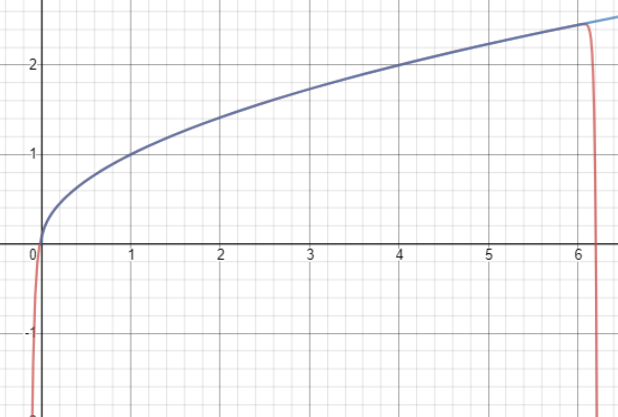
\includegraphics[scale=1]{sqrt}
\end{figure}

The blue curve is the actual function, and the red curve is the polynomial approximation, of course. As you can see, the polynomial breaks down around $x=6$ and $x=0$. You could find using some tedious math to get the actual radius of convergence to be $r=3$, or you could just tell that since $\sqrt{x}$ is not differentiable at $0$ the series fails to converge beyond that point. So from observation we can tell the radius of convergence for the square root is just the value $a$.

Then consider the Maclaurin series for $\frac{1}{1+x^2}$:

$$\frac{1}{1+x^2} \approx T_n(x) = \sum_{k=0}^{n}\left(-1\right)^{k}x^{2k}$$

For large n the approximation looks like so:

\begin{figure}[h]
\centering
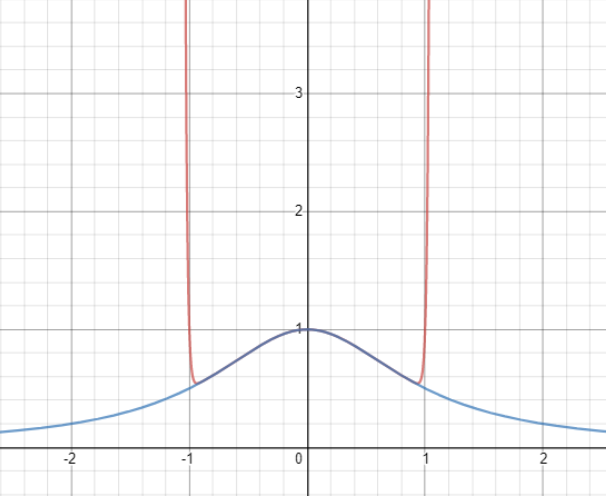
\includegraphics[scale=1]{darctan}
\end{figure}

With a little math, we can find that the radius of convergence is 1, but this is not apparent from the graph because there are no spots where the original function is not differentiable... on the reals at least. Consider the same original function $\frac{1}{1+x^2}$ but in the complex plane, so it would be $\frac{1}{1+z^2}$. Taylor works just as well in the complex plane, but now we can see that the closest point where the function is no longer differentiable (nor existent for that matter) is at $z=i$, and the distance from the center of the polynomial we made, $0$, to $i$, is $1$. Hence the radius of convergence is $1$. In general this is true - the radius of convergence of a Taylor series centered at $a$ is the distance from the point $a$ to the nearest point $z_0$ for which the original function is not holomorphic (or complex differentiable) in the complex plane.

\begin{flushright}
Sai Sivakumar
\end{flushright}

\newpage

$$\left[\sum_{k=0}^n\frac{f^{k}}{k!}(x-a)^k \right]+ R_n(x)$$
$$R_n(x) = \frac{f^{n+1}(z)}{(n+1)!}(x-a)^{n+1}, z\in[a,x]$$
1.
$$R_n(x) = \int_a^x \frac{f^{n+1}(t)}{n!}(t-a)^{n}\dd{t}$$
$$m = \min_{t\in[a,x]} f^{n+1}(t)$$
$$M = \max_{t\in[a,x]} f^{n+1}(t)$$
$$I = \int_a^x \frac{(t-a)^n}{n!} = \frac{(x-a)^{n+1}}{(n+1)!}$$
$$\int_a^x \frac{f^{n+1}(t)}{n!}(t-a)^{n}\dd{t} \in [mI,MI]$$
$$\max_{z\in[a,x]} R_n(x) = \frac{f^{n+1}(z)}{(n+1)!}(x-a)^{n+1}$$
As a side note we require $f^{n+1}$ to be absolutely continuous.

2.
$$R_n(x) = \int_a^x \frac{f^{n+1}(t)}{n!}(t-a)^{n}\dd{t}$$
$$R_n(x) = {(x-a)}\frac{1}{x-a}\int_a^x \frac{f^{n+1}(t)}{n!}(t-a)^{n}\dd{t}$$
$$R_n(x) = \frac{f^{n+1}(c)}{n!}(c-a)^n(x-a), {c\in[a,x]}$$

\end{document}